\documentclass[1p]{elsarticle_modified}
%\bibliographystyle{elsarticle-num}

%\usepackage[colorlinks]{hyperref}
%\usepackage{abbrmath_seonhwa} %\Abb, \Ascr, \Acal ,\Abf, \Afrak
\usepackage{amsfonts}
\usepackage{amssymb}
\usepackage{amsmath}
\usepackage{amsthm}
\usepackage{scalefnt}
\usepackage{amsbsy}
\usepackage{kotex}
\usepackage{caption}
\usepackage{subfig}
\usepackage{color}
\usepackage{graphicx}
\usepackage{xcolor} %% white, black, red, green, blue, cyan, magenta, yellow
\usepackage{float}
\usepackage{setspace}
\usepackage{hyperref}

\usepackage{tikz}
\usetikzlibrary{arrows}

\usepackage{multirow}
\usepackage{array} % fixed length table
\usepackage{hhline}

%%%%%%%%%%%%%%%%%%%%%
\makeatletter
\renewcommand*\env@matrix[1][\arraystretch]{%
	\edef\arraystretch{#1}%
	\hskip -\arraycolsep
	\let\@ifnextchar\new@ifnextchar
	\array{*\c@MaxMatrixCols c}}
\makeatother %https://tex.stackexchange.com/questions/14071/how-can-i-increase-the-line-spacing-in-a-matrix
%%%%%%%%%%%%%%%

\usepackage[normalem]{ulem}

\newcommand{\msout}[1]{\ifmmode\text{\sout{\ensuremath{#1}}}\else\sout{#1}\fi}
%SOURCE: \msout is \stkout macro in https://tex.stackexchange.com/questions/20609/strikeout-in-math-mode

\newcommand{\cancel}[1]{
	\ifmmode
	{\color{red}\msout{#1}}
	\else
	{\color{red}\sout{#1}}
	\fi
}

\newcommand{\add}[1]{
	{\color{blue}\uwave{#1}}
}

\newcommand{\replace}[2]{
	\ifmmode
	{\color{red}\msout{#1}}{\color{blue}\uwave{#2}}
	\else
	{\color{red}\sout{#1}}{\color{blue}\uwave{#2}}
	\fi
}

\newcommand{\Sol}{\mathcal{S}} %segment
\newcommand{\D}{D} %diagram
\newcommand{\A}{\mathcal{A}} %arc


%%%%%%%%%%%%%%%%%%%%%%%%%%%%%5 test

\def\sl{\operatorname{\textup{SL}}(2,\Cbb)}
\def\psl{\operatorname{\textup{PSL}}(2,\Cbb)}
\def\quan{\mkern 1mu \triangleright \mkern 1mu}

\theoremstyle{definition}
\newtheorem{thm}{Theorem}[section]
\newtheorem{prop}[thm]{Proposition}
\newtheorem{lem}[thm]{Lemma}
\newtheorem{ques}[thm]{Question}
\newtheorem{cor}[thm]{Corollary}
\newtheorem{defn}[thm]{Definition}
\newtheorem{exam}[thm]{Example}
\newtheorem{rmk}[thm]{Remark}
\newtheorem{alg}[thm]{Algorithm}

\newcommand{\I}{\sqrt{-1}}
\begin{document}

%\begin{frontmatter}
%
%\title{Boundary parabolic representations of knots up to 8 crossings}
%
%%% Group authors per affiliation:
%\author{Yunhi Cho} 
%\address{Department of Mathematics, University of Seoul, Seoul, Korea}
%\ead{yhcho@uos.ac.kr}
%
%
%\author{Seonhwa Kim} %\fnref{s_kim}}
%\address{Center for Geometry and Physics, Institute for Basic Science, Pohang, 37673, Korea}
%\ead{ryeona17@ibs.re.kr}
%
%\author{Hyuk Kim}
%\address{Department of Mathematical Sciences, Seoul National University, Seoul 08826, Korea}
%\ead{hyukkim@snu.ac.kr}
%
%\author{Seokbeom Yoon}
%\address{Department of Mathematical Sciences, Seoul National University, Seoul, 08826,  Korea}
%\ead{sbyoon15@snu.ac.kr}
%
%\begin{abstract}
%We find all boundary parabolic representation of knots up to 8 crossings.
%
%\end{abstract}
%\begin{keyword}
%    \MSC[2010] 57M25 
%\end{keyword}
%
%\end{frontmatter}

%\linenumbers
%\tableofcontents
%
\newcommand\colored[1]{\textcolor{white}{\rule[-0.35ex]{0.8em}{1.4ex}}\kern-0.8em\color{red} #1}%
%\newcommand\colored[1]{\textcolor{white}{ #1}\kern-2.17ex	\textcolor{white}{ #1}\kern-1.81ex	\textcolor{white}{ #1}\kern-2.15ex\color{red}#1	}

{\Large $\underline{12a_{0159}~(K12a_{0159})}$}

\setlength{\tabcolsep}{10pt}
\renewcommand{\arraystretch}{1.6}
\vspace{1cm}\begin{tabular}{m{100pt}>{\centering\arraybackslash}m{274pt}}
\multirow{5}{120pt}{
	\centering
	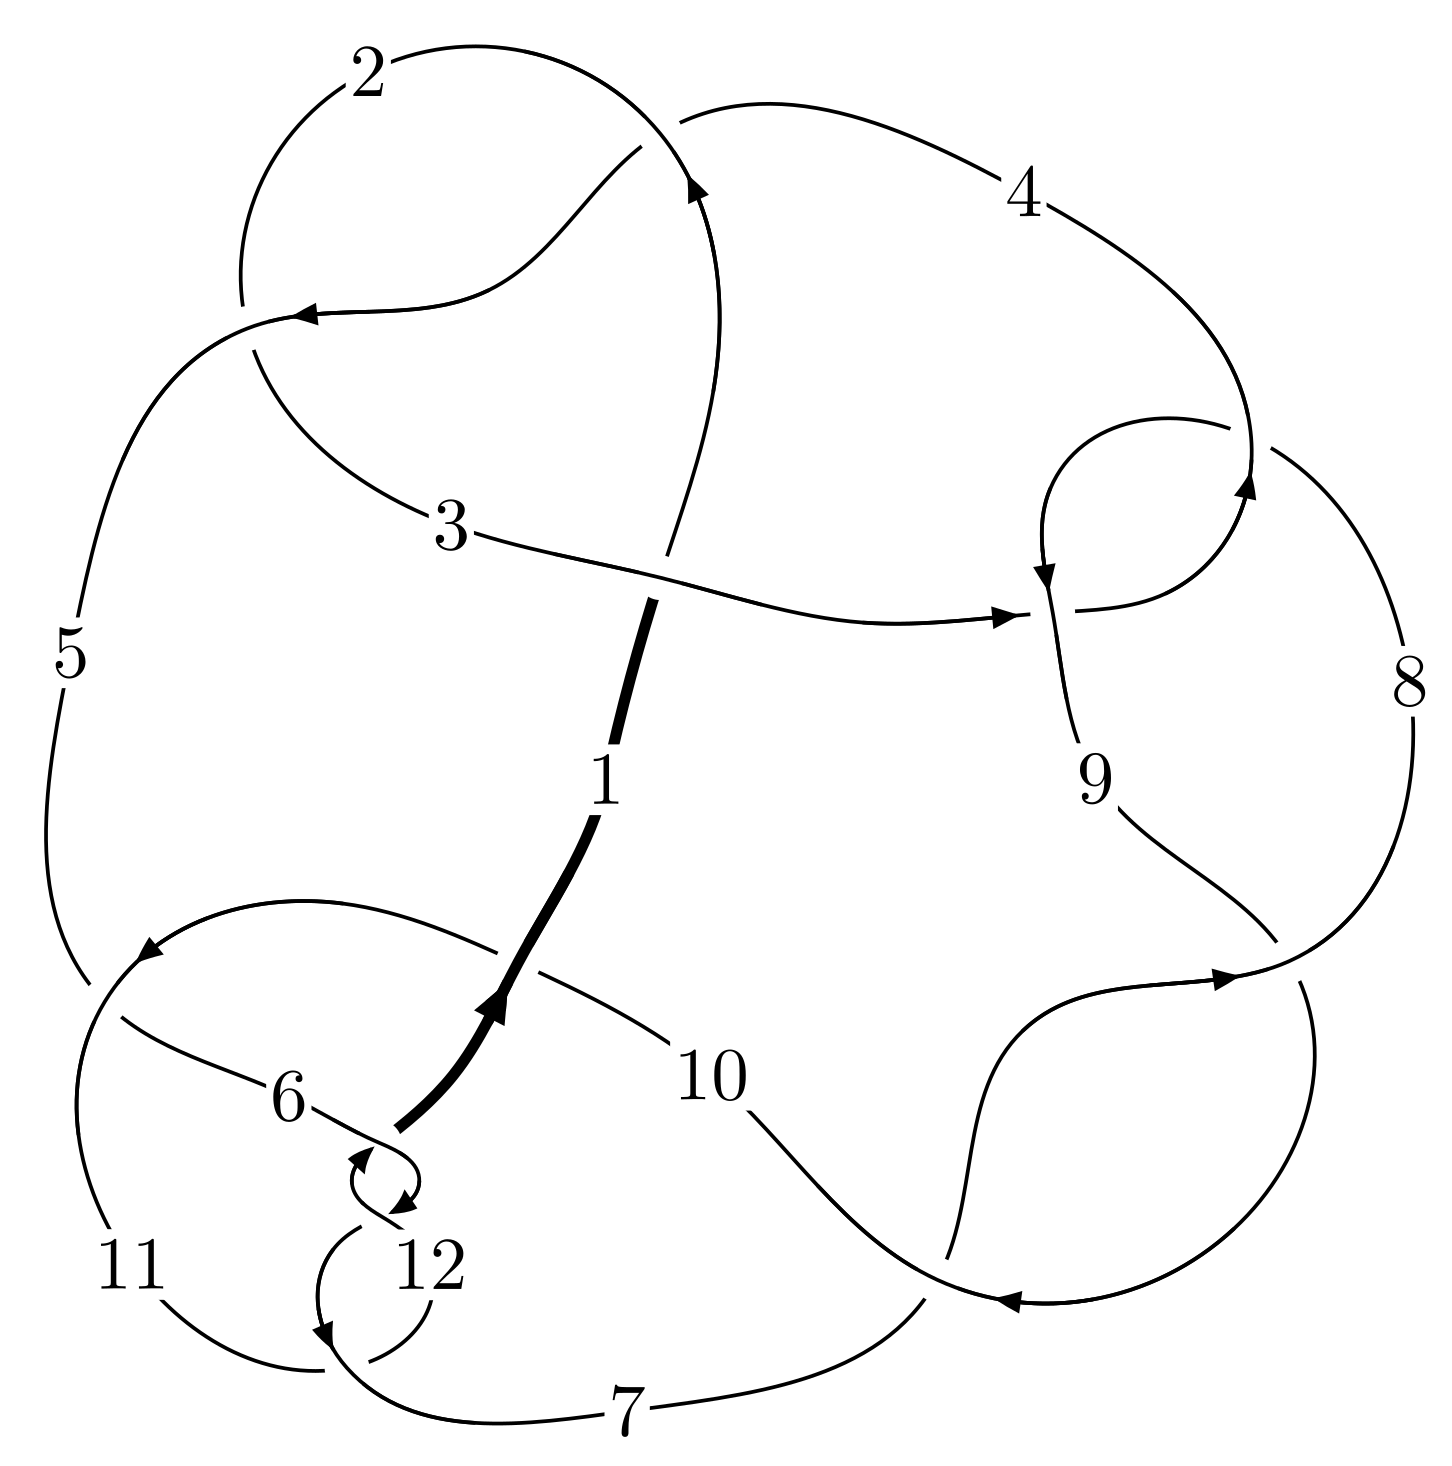
\includegraphics[width=112pt]{../../../GIT/diagram.site/Diagrams/png/960_12a_0159.png}\\
\ \ \ A knot diagram\footnotemark}&
\allowdisplaybreaks
\textbf{Linearized knot diagam} \\
\cline{2-2}
 &
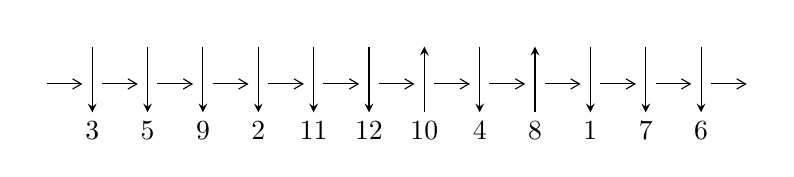
\begin{tikzpicture}[x=20pt, y=17pt]
	% nodes
	\node (C0) at (0, 0) {};
	\node (C1) at (1, 0) {};
	\node (C1U) at (1, +1) {};
	\node (C1D) at (1, -1) {3};

	\node (C2) at (2, 0) {};
	\node (C2U) at (2, +1) {};
	\node (C2D) at (2, -1) {5};

	\node (C3) at (3, 0) {};
	\node (C3U) at (3, +1) {};
	\node (C3D) at (3, -1) {9};

	\node (C4) at (4, 0) {};
	\node (C4U) at (4, +1) {};
	\node (C4D) at (4, -1) {2};

	\node (C5) at (5, 0) {};
	\node (C5U) at (5, +1) {};
	\node (C5D) at (5, -1) {11};

	\node (C6) at (6, 0) {};
	\node (C6U) at (6, +1) {};
	\node (C6D) at (6, -1) {12};

	\node (C7) at (7, 0) {};
	\node (C7U) at (7, +1) {};
	\node (C7D) at (7, -1) {10};

	\node (C8) at (8, 0) {};
	\node (C8U) at (8, +1) {};
	\node (C8D) at (8, -1) {4};

	\node (C9) at (9, 0) {};
	\node (C9U) at (9, +1) {};
	\node (C9D) at (9, -1) {8};

	\node (C10) at (10, 0) {};
	\node (C10U) at (10, +1) {};
	\node (C10D) at (10, -1) {1};

	\node (C11) at (11, 0) {};
	\node (C11U) at (11, +1) {};
	\node (C11D) at (11, -1) {7};

	\node (C12) at (12, 0) {};
	\node (C12U) at (12, +1) {};
	\node (C12D) at (12, -1) {6};
	\node (C13) at (13, 0) {};

	% arrows
	\draw[->,>={angle 60}]
	(C0) edge (C1) (C1) edge (C2) (C2) edge (C3) (C3) edge (C4) (C4) edge (C5) (C5) edge (C6) (C6) edge (C7) (C7) edge (C8) (C8) edge (C9) (C9) edge (C10) (C10) edge (C11) (C11) edge (C12) (C12) edge (C13) ;	\draw[->,>=stealth]
	(C1U) edge (C1D) (C2U) edge (C2D) (C3U) edge (C3D) (C4U) edge (C4D) (C5U) edge (C5D) (C6U) edge (C6D) (C7D) edge (C7U) (C8U) edge (C8D) (C9D) edge (C9U) (C10U) edge (C10D) (C11U) edge (C11D) (C12U) edge (C12D) ;
	\end{tikzpicture} \\
\hhline{~~} \\& 
\textbf{Solving Sequence} \\ \cline{2-2} 
 &
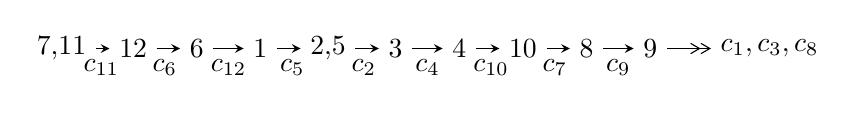
\begin{tikzpicture}[x=23pt, y=7pt]
	% node
	\node (A0) at (-1/8, 0) {7,11};
	\node (A1) at (1, 0) {12};
	\node (A2) at (2, 0) {6};
	\node (A3) at (3, 0) {1};
	\node (A4) at (65/16, 0) {2,5};
	\node (A5) at (41/8, 0) {3};
	\node (A6) at (49/8, 0) {4};
	\node (A7) at (57/8, 0) {10};
	\node (A8) at (65/8, 0) {8};
	\node (A9) at (73/8, 0) {9};
	\node (C1) at (1/2, -1) {$c_{11}$};
	\node (C2) at (3/2, -1) {$c_{6}$};
	\node (C3) at (5/2, -1) {$c_{12}$};
	\node (C4) at (7/2, -1) {$c_{5}$};
	\node (C5) at (37/8, -1) {$c_{2}$};
	\node (C6) at (45/8, -1) {$c_{4}$};
	\node (C7) at (53/8, -1) {$c_{10}$};
	\node (C8) at (61/8, -1) {$c_{7}$};
	\node (C9) at (69/8, -1) {$c_{9}$};
	\node (A10) at (11, 0) {$c_{1},c_{3},c_{8}$};

	% edge
	\draw[->,>=stealth]	
	(A0) edge (A1) (A1) edge (A2) (A2) edge (A3) (A3) edge (A4) (A4) edge (A5) (A5) edge (A6) (A6) edge (A7) (A7) edge (A8) (A8) edge (A9) ;
	\draw[->>,>={angle 60}]	
	(A9) edge (A10);
\end{tikzpicture} \\ 

\end{tabular} \\

\footnotetext{
The image of knot diagram is generated by the software ``\textbf{Draw programme}" developed by Andrew Bartholomew(\url{http://www.layer8.co.uk/maths/draw/index.htm\#Running-draw}), where we modified some parts for our purpose(\url{https://github.com/CATsTAILs/LinksPainter}).
}\phantom \\ \newline 
\centering \textbf{Ideals for irreducible components\footnotemark of $X_{\text{par}}$} 
 
\begin{align*}
I^u_{1}&=\langle 
u^{80}-2 u^{79}+\cdots+b-1,\;- u^{45}-20 u^{43}+\cdots+a-2,\;u^{81}-2 u^{80}+\cdots- u+1\rangle \\
I^u_{2}&=\langle 
-2 u^2+b-2 u-2,\;- u^2+a-1,\;u^3+u^2+2 u+1\rangle \\
\\
\end{align*}
\raggedright * 2 irreducible components of $\dim_{\mathbb{C}}=0$, with total 84 representations.\\
\footnotetext{All coefficients of polynomials are rational numbers. But the coefficients are sometimes approximated in decimal forms when there is not enough margin.}
\newpage
\renewcommand{\arraystretch}{1}
\centering \section*{I. $I^u_{1}= \langle u^{80}-2 u^{79}+\cdots+b-1,\;- u^{45}-20 u^{43}+\cdots+a-2,\;u^{81}-2 u^{80}+\cdots- u+1 \rangle$}
\flushleft \textbf{(i) Arc colorings}\\
\begin{tabular}{m{7pt} m{180pt} m{7pt} m{180pt} }
\flushright $a_{7}=$&$\begin{pmatrix}0\\u\end{pmatrix}$ \\
\flushright $a_{11}=$&$\begin{pmatrix}1\\0\end{pmatrix}$ \\
\flushright $a_{12}=$&$\begin{pmatrix}1\\u^2\end{pmatrix}$ \\
\flushright $a_{6}=$&$\begin{pmatrix}u\\u^3+u\end{pmatrix}$ \\
\flushright $a_{1}=$&$\begin{pmatrix}u^2+1\\u^4+2 u^2\end{pmatrix}$ \\
\flushright $a_{2}=$&$\begin{pmatrix}u^{45}+20 u^{43}+\cdots- u+2\\- u^{80}+2 u^{79}+\cdots- u+1\end{pmatrix}$ \\
\flushright $a_{5}=$&$\begin{pmatrix}u^3+2 u\\u^3+u\end{pmatrix}$ \\
\flushright $a_{3}=$&$\begin{pmatrix}u^{80}- u^{79}+\cdots-2 u+1\\- u^{53}-23 u^{51}+\cdots+4 u^2- u\end{pmatrix}$ \\
\flushright $a_{4}=$&$\begin{pmatrix}u^{80}- u^{79}+\cdots+3 u-2\\2 u^{80}-4 u^{79}+\cdots+2 u-2\end{pmatrix}$ \\
\flushright $a_{10}=$&$\begin{pmatrix}- u^6-3 u^4-2 u^2+1\\- u^8-4 u^6-4 u^4\end{pmatrix}$ \\
\flushright $a_{8}=$&$\begin{pmatrix}u^{13}+6 u^{11}+13 u^9+10 u^7-2 u^5-4 u^3+u\\u^{15}+7 u^{13}+18 u^{11}+19 u^9+4 u^7-4 u^5+u\end{pmatrix}$ \\
\flushright $a_{9}=$&$\begin{pmatrix}- u^{20}-9 u^{18}+\cdots- u^2+1\\- u^{22}-10 u^{20}+\cdots-6 u^4+u^2\end{pmatrix}$\\&\end{tabular}
\flushleft \textbf{(ii) Obstruction class $= -1$}\\~\\
\flushleft \textbf{(iii) Cusp Shapes $= u^{80}-2 u^{79}+\cdots+14 u-13$}\\~\\
\newpage\renewcommand{\arraystretch}{1}
\flushleft \textbf{(iv) u-Polynomials at the component}\newline \\
\begin{tabular}{m{50pt}|m{274pt}}
Crossings & \hspace{64pt}u-Polynomials at each crossing \\
\hline $$\begin{aligned}c_{1}\end{aligned}$$&$\begin{aligned}
&u^{81}+46 u^{80}+\cdots+24 u+1
\end{aligned}$\\
\hline $$\begin{aligned}c_{2},c_{4}\end{aligned}$$&$\begin{aligned}
&u^{81}-4 u^{80}+\cdots-12 u^2+1
\end{aligned}$\\
\hline $$\begin{aligned}c_{3},c_{8}\end{aligned}$$&$\begin{aligned}
&u^{81}- u^{80}+\cdots+12 u+8
\end{aligned}$\\
\hline $$\begin{aligned}c_{5}\end{aligned}$$&$\begin{aligned}
&u^{81}+2 u^{80}+\cdots-43 u+17
\end{aligned}$\\
\hline $$\begin{aligned}c_{6},c_{11},c_{12}\end{aligned}$$&$\begin{aligned}
&u^{81}-2 u^{80}+\cdots- u+1
\end{aligned}$\\
\hline $$\begin{aligned}c_{7},c_{9}\end{aligned}$$&$\begin{aligned}
&u^{81}-21 u^{80}+\cdots-752 u+64
\end{aligned}$\\
\hline $$\begin{aligned}c_{10}\end{aligned}$$&$\begin{aligned}
&u^{81}-20 u^{80}+\cdots-343 u+19
\end{aligned}$\\
\hline
\end{tabular}\\~\\
\newpage\renewcommand{\arraystretch}{1}
\flushleft \textbf{(v) Riley Polynomials at the component}\newline \\
\begin{tabular}{m{50pt}|m{274pt}}
Crossings & \hspace{64pt}Riley Polynomials at each crossing \\
\hline $$\begin{aligned}c_{1}\end{aligned}$$&$\begin{aligned}
&y^{81}-18 y^{80}+\cdots+460 y-1
\end{aligned}$\\
\hline $$\begin{aligned}c_{2},c_{4}\end{aligned}$$&$\begin{aligned}
&y^{81}-46 y^{80}+\cdots+24 y-1
\end{aligned}$\\
\hline $$\begin{aligned}c_{3},c_{8}\end{aligned}$$&$\begin{aligned}
&y^{81}+21 y^{80}+\cdots-752 y-64
\end{aligned}$\\
\hline $$\begin{aligned}c_{5}\end{aligned}$$&$\begin{aligned}
&y^{81}-8 y^{80}+\cdots-1245 y-289
\end{aligned}$\\
\hline $$\begin{aligned}c_{6},c_{11},c_{12}\end{aligned}$$&$\begin{aligned}
&y^{81}+72 y^{80}+\cdots+11 y-1
\end{aligned}$\\
\hline $$\begin{aligned}c_{7},c_{9}\end{aligned}$$&$\begin{aligned}
&y^{81}+73 y^{80}+\cdots+118016 y-4096
\end{aligned}$\\
\hline $$\begin{aligned}c_{10}\end{aligned}$$&$\begin{aligned}
&y^{81}+4 y^{80}+\cdots-14021 y-361
\end{aligned}$\\
\hline
\end{tabular}\\~\\
\newpage\flushleft \textbf{(vi) Complex Volumes and Cusp Shapes}
$$\begin{array}{c|c|c}  
\text{Solutions to }I^u_{1}& \I (\text{vol} + \sqrt{-1}CS) & \text{Cusp shape}\\
 \hline 
\begin{aligned}
u &= -0.303170 + 0.945098 I \\
a &= -0.25327 - 2.53154 I \\
b &= -0.672053 + 0.231950 I\end{aligned}
 & -5.77830 + 7.46778 I & \phantom{-0.000000 } 0 \\ \hline\begin{aligned}
u &= -0.303170 - 0.945098 I \\
a &= -0.25327 + 2.53154 I \\
b &= -0.672053 - 0.231950 I\end{aligned}
 & -5.77830 - 7.46778 I & \phantom{-0.000000 } 0 \\ \hline\begin{aligned}
u &= -0.247473 + 0.919700 I \\
a &= \phantom{-}0.535003 - 0.348621 I \\
b &= -0.604404 - 0.273353 I\end{aligned}
 & -2.29387 + 2.82287 I & \phantom{-0.000000 } 0 \\ \hline\begin{aligned}
u &= -0.247473 - 0.919700 I \\
a &= \phantom{-}0.535003 + 0.348621 I \\
b &= -0.604404 + 0.273353 I\end{aligned}
 & -2.29387 - 2.82287 I & \phantom{-0.000000 } 0 \\ \hline\begin{aligned}
u &= \phantom{-}0.270652 + 0.876959 I \\
a &= \phantom{-}0.04945 + 2.65701 I \\
b &= -0.360007 - 0.114986 I\end{aligned}
 & -6.07844 - 1.32566 I & -11.28844 + 0. I\phantom{ +0.000000I} \\ \hline\begin{aligned}
u &= \phantom{-}0.270652 - 0.876959 I \\
a &= \phantom{-}0.04945 - 2.65701 I \\
b &= -0.360007 + 0.114986 I\end{aligned}
 & -6.07844 + 1.32566 I & -11.28844 + 0. I\phantom{ +0.000000I} \\ \hline\begin{aligned}
u &= -0.281291 + 0.845764 I \\
a &= \phantom{-}1.02701 + 2.86058 I \\
b &= \phantom{-}1.361880 - 0.185998 I\end{aligned}
 & -6.03068 - 1.59014 I & -11.18638 + 0. I\phantom{ +0.000000I} \\ \hline\begin{aligned}
u &= -0.281291 - 0.845764 I \\
a &= \phantom{-}1.02701 - 2.86058 I \\
b &= \phantom{-}1.361880 + 0.185998 I\end{aligned}
 & -6.03068 + 1.59014 I & -11.18638 + 0. I\phantom{ +0.000000I} \\ \hline\begin{aligned}
u &= \phantom{-}0.346370 + 0.811440 I \\
a &= \phantom{-}0.82935 - 2.96214 I \\
b &= \phantom{-}1.341850 - 0.112388 I\end{aligned}
 & -5.49518 + 7.85390 I & -10.12792 - 4.44787 I \\ \hline\begin{aligned}
u &= \phantom{-}0.346370 - 0.811440 I \\
a &= \phantom{-}0.82935 + 2.96214 I \\
b &= \phantom{-}1.341850 + 0.112388 I\end{aligned}
 & -5.49518 - 7.85390 I & -10.12792 + 4.44787 I\\
 \hline 
 \end{array}$$\newpage$$\begin{array}{c|c|c}  
\text{Solutions to }I^u_{1}& \I (\text{vol} + \sqrt{-1}CS) & \text{Cusp shape}\\
 \hline 
\begin{aligned}
u &= \phantom{-}0.289974 + 0.797976 I \\
a &= \phantom{-}0.674590 + 0.182571 I \\
b &= -0.432715 + 0.241146 I\end{aligned}
 & -2.12042 + 3.02576 I & -7.01113 - 1.60503 I \\ \hline\begin{aligned}
u &= \phantom{-}0.289974 - 0.797976 I \\
a &= \phantom{-}0.674590 - 0.182571 I \\
b &= -0.432715 - 0.241146 I\end{aligned}
 & -2.12042 - 3.02576 I & -7.01113 + 1.60503 I \\ \hline\begin{aligned}
u &= \phantom{-}0.752560 + 0.251187 I \\
a &= -4.05489 + 0.08335 I \\
b &= -3.13602 - 0.13798 I\end{aligned}
 & -7.35624 - 11.91150 I & -12.6732 + 9.0421 I \\ \hline\begin{aligned}
u &= \phantom{-}0.752560 - 0.251187 I \\
a &= -4.05489 - 0.08335 I \\
b &= -3.13602 + 0.13798 I\end{aligned}
 & -7.35624 + 11.91150 I & -12.6732 - 9.0421 I \\ \hline\begin{aligned}
u &= -0.219870 + 1.189280 I \\
a &= -0.413984 - 1.123960 I \\
b &= -1.04512 + 1.25784 I\end{aligned}
 & \phantom{-}1.12936 + 4.60878 I & \phantom{-0.000000 } 0 \\ \hline\begin{aligned}
u &= -0.219870 - 1.189280 I \\
a &= -0.413984 + 1.123960 I \\
b &= -1.04512 - 1.25784 I\end{aligned}
 & \phantom{-}1.12936 - 4.60878 I & \phantom{-0.000000 } 0 \\ \hline\begin{aligned}
u &= -0.755022 + 0.193964 I \\
a &= \phantom{-}3.02006 - 0.86714 I \\
b &= \phantom{-}2.29261 - 0.23467 I\end{aligned}
 & -8.11616 - 3.50154 I & -14.0566 + 2.3476 I \\ \hline\begin{aligned}
u &= -0.755022 - 0.193964 I \\
a &= \phantom{-}3.02006 + 0.86714 I \\
b &= \phantom{-}2.29261 + 0.23467 I\end{aligned}
 & -8.11616 + 3.50154 I & -14.0566 - 2.3476 I \\ \hline\begin{aligned}
u &= \phantom{-}0.735753 + 0.244806 I \\
a &= \phantom{-}0.373365 + 0.673804 I \\
b &= \phantom{-}0.339700 + 0.852192 I\end{aligned}
 & -3.98935 - 6.91470 I & -9.71071 + 6.26433 I \\ \hline\begin{aligned}
u &= \phantom{-}0.735753 - 0.244806 I \\
a &= \phantom{-}0.373365 - 0.673804 I \\
b &= \phantom{-}0.339700 - 0.852192 I\end{aligned}
 & -3.98935 + 6.91470 I & -9.71071 - 6.26433 I\\
 \hline 
 \end{array}$$\newpage$$\begin{array}{c|c|c}  
\text{Solutions to }I^u_{1}& \I (\text{vol} + \sqrt{-1}CS) & \text{Cusp shape}\\
 \hline 
\begin{aligned}
u &= -0.738922 + 0.231068 I \\
a &= -4.21182 - 0.51748 I \\
b &= -3.24525 - 0.13613 I\end{aligned}
 & -8.03409 + 5.47694 I & -13.9444 - 4.7227 I \\ \hline\begin{aligned}
u &= -0.738922 - 0.231068 I \\
a &= -4.21182 + 0.51748 I \\
b &= -3.24525 + 0.13613 I\end{aligned}
 & -8.03409 - 5.47694 I & -13.9444 + 4.7227 I \\ \hline\begin{aligned}
u &= \phantom{-}0.737771 + 0.220516 I \\
a &= \phantom{-}2.94150 + 1.15749 I \\
b &= \phantom{-}2.23096 + 0.39996 I\end{aligned}
 & -8.17510 - 2.53314 I & -14.1431 + 3.4480 I \\ \hline\begin{aligned}
u &= \phantom{-}0.737771 - 0.220516 I \\
a &= \phantom{-}2.94150 - 1.15749 I \\
b &= \phantom{-}2.23096 - 0.39996 I\end{aligned}
 & -8.17510 + 2.53314 I & -14.1431 - 3.4480 I \\ \hline\begin{aligned}
u &= -0.729425 + 0.205364 I \\
a &= \phantom{-}0.667285 - 0.705734 I \\
b &= \phantom{-}0.523998 - 0.848028 I\end{aligned}
 & -4.51674 + 0.94829 I & -10.85953 - 1.20447 I \\ \hline\begin{aligned}
u &= -0.729425 - 0.205364 I \\
a &= \phantom{-}0.667285 + 0.705734 I \\
b &= \phantom{-}0.523998 + 0.848028 I\end{aligned}
 & -4.51674 - 0.94829 I & -10.85953 + 1.20447 I \\ \hline\begin{aligned}
u &= \phantom{-}0.059550 + 1.270820 I \\
a &= \phantom{-}0.365987 + 0.264958 I \\
b &= -0.87854 - 2.17817 I\end{aligned}
 & \phantom{-}0.489163 - 1.113280 I & \phantom{-0.000000 } 0 \\ \hline\begin{aligned}
u &= \phantom{-}0.059550 - 1.270820 I \\
a &= \phantom{-}0.365987 - 0.264958 I \\
b &= -0.87854 + 2.17817 I\end{aligned}
 & \phantom{-}0.489163 + 1.113280 I & \phantom{-0.000000 } 0 \\ \hline\begin{aligned}
u &= \phantom{-}0.644664 + 0.307621 I \\
a &= -2.00622 + 0.71203 I \\
b &= -1.87711 + 0.34103 I\end{aligned}
 & \phantom{-}0.80619 - 6.96807 I & -7.43117 + 9.89323 I \\ \hline\begin{aligned}
u &= \phantom{-}0.644664 - 0.307621 I \\
a &= -2.00622 - 0.71203 I \\
b &= -1.87711 - 0.34103 I\end{aligned}
 & \phantom{-}0.80619 + 6.96807 I & -7.43117 - 9.89323 I\\
 \hline 
 \end{array}$$\newpage$$\begin{array}{c|c|c}  
\text{Solutions to }I^u_{1}& \I (\text{vol} + \sqrt{-1}CS) & \text{Cusp shape}\\
 \hline 
\begin{aligned}
u &= -0.686300 + 0.060020 I \\
a &= \phantom{-}2.02694 - 0.13374 I \\
b &= \phantom{-}1.69352 + 0.12385 I\end{aligned}
 & -2.25856 - 1.25913 I & -10.34603 + 5.18490 I \\ \hline\begin{aligned}
u &= -0.686300 - 0.060020 I \\
a &= \phantom{-}2.02694 + 0.13374 I \\
b &= \phantom{-}1.69352 - 0.12385 I\end{aligned}
 & -2.25856 + 1.25913 I & -10.34603 - 5.18490 I \\ \hline\begin{aligned}
u &= -0.261073 + 1.293880 I \\
a &= -0.731555 - 0.804325 I \\
b &= -1.88353 + 0.90574 I\end{aligned}
 & \phantom{-}1.94624 + 2.16799 I & \phantom{-0.000000 } 0 \\ \hline\begin{aligned}
u &= -0.261073 - 1.293880 I \\
a &= -0.731555 + 0.804325 I \\
b &= -1.88353 - 0.90574 I\end{aligned}
 & \phantom{-}1.94624 - 2.16799 I & \phantom{-0.000000 } 0 \\ \hline\begin{aligned}
u &= -0.139892 + 1.312790 I \\
a &= -0.595311 - 0.245748 I \\
b &= -0.507967 + 0.428038 I\end{aligned}
 & \phantom{-}3.30113 + 2.08996 I & \phantom{-0.000000 } 0 \\ \hline\begin{aligned}
u &= -0.139892 - 1.312790 I \\
a &= -0.595311 + 0.245748 I \\
b &= -0.507967 - 0.428038 I\end{aligned}
 & \phantom{-}3.30113 - 2.08996 I & \phantom{-0.000000 } 0 \\ \hline\begin{aligned}
u &= \phantom{-}0.580222 + 0.318959 I \\
a &= \phantom{-}0.515067 - 0.446557 I \\
b &= \phantom{-}0.337288 + 0.302817 I\end{aligned}
 & \phantom{-}2.24419 - 2.41279 I & -3.70773 + 4.77664 I \\ \hline\begin{aligned}
u &= \phantom{-}0.580222 - 0.318959 I \\
a &= \phantom{-}0.515067 + 0.446557 I \\
b &= \phantom{-}0.337288 - 0.302817 I\end{aligned}
 & \phantom{-}2.24419 + 2.41279 I & -3.70773 - 4.77664 I \\ \hline\begin{aligned}
u &= \phantom{-}0.389422 + 0.511342 I \\
a &= \phantom{-}0.74082 - 2.00362 I \\
b &= \phantom{-}0.637861 - 0.068396 I\end{aligned}
 & \phantom{-}1.73888 + 3.42569 I & -4.42143 - 3.64386 I \\ \hline\begin{aligned}
u &= \phantom{-}0.389422 - 0.511342 I \\
a &= \phantom{-}0.74082 + 2.00362 I \\
b &= \phantom{-}0.637861 + 0.068396 I\end{aligned}
 & \phantom{-}1.73888 - 3.42569 I & -4.42143 + 3.64386 I\\
 \hline 
 \end{array}$$\newpage$$\begin{array}{c|c|c}  
\text{Solutions to }I^u_{1}& \I (\text{vol} + \sqrt{-1}CS) & \text{Cusp shape}\\
 \hline 
\begin{aligned}
u &= -0.026303 + 1.378390 I \\
a &= \phantom{-}0.535969 - 0.756911 I \\
b &= -0.79945 - 2.55508 I\end{aligned}
 & \phantom{-}0.535961 - 1.295870 I & \phantom{-0.000000 } 0 \\ \hline\begin{aligned}
u &= -0.026303 - 1.378390 I \\
a &= \phantom{-}0.535969 + 0.756911 I \\
b &= -0.79945 + 2.55508 I\end{aligned}
 & \phantom{-}0.535961 + 1.295870 I & \phantom{-0.000000 } 0 \\ \hline\begin{aligned}
u &= -0.570968 + 0.236387 I \\
a &= -1.18110 - 2.38772 I \\
b &= -1.46997 - 1.37738 I\end{aligned}
 & -1.74111 + 2.68316 I & -11.58262 - 7.10742 I \\ \hline\begin{aligned}
u &= -0.570968 - 0.236387 I \\
a &= -1.18110 + 2.38772 I \\
b &= -1.46997 + 1.37738 I\end{aligned}
 & -1.74111 - 2.68316 I & -11.58262 + 7.10742 I \\ \hline\begin{aligned}
u &= \phantom{-}0.214093 + 1.367380 I \\
a &= -0.964506 + 0.271292 I \\
b &= -2.25687 - 1.90809 I\end{aligned}
 & \phantom{-}2.33114 - 3.63921 I & \phantom{-0.000000 } 0 \\ \hline\begin{aligned}
u &= \phantom{-}0.214093 - 1.367380 I \\
a &= -0.964506 - 0.271292 I \\
b &= -2.25687 + 1.90809 I\end{aligned}
 & \phantom{-}2.33114 + 3.63921 I & \phantom{-0.000000 } 0 \\ \hline\begin{aligned}
u &= -0.184866 + 1.372520 I \\
a &= -0.150775 - 1.243160 I \\
b &= -1.290460 - 0.203550 I\end{aligned}
 & \phantom{-}4.04253 + 2.04762 I & \phantom{-0.000000 } 0 \\ \hline\begin{aligned}
u &= -0.184866 - 1.372520 I \\
a &= -0.150775 + 1.243160 I \\
b &= -1.290460 + 0.203550 I\end{aligned}
 & \phantom{-}4.04253 - 2.04762 I & \phantom{-0.000000 } 0 \\ \hline\begin{aligned}
u &= \phantom{-}0.454129 + 0.406277 I \\
a &= \phantom{-}0.140115 + 0.400135 I \\
b &= -0.588763 + 0.305661 I\end{aligned}
 & \phantom{-}2.70212 - 0.89217 I & -1.88644 + 3.94554 I \\ \hline\begin{aligned}
u &= \phantom{-}0.454129 - 0.406277 I \\
a &= \phantom{-}0.140115 - 0.400135 I \\
b &= -0.588763 - 0.305661 I\end{aligned}
 & \phantom{-}2.70212 + 0.89217 I & -1.88644 - 3.94554 I\\
 \hline 
 \end{array}$$\newpage$$\begin{array}{c|c|c}  
\text{Solutions to }I^u_{1}& \I (\text{vol} + \sqrt{-1}CS) & \text{Cusp shape}\\
 \hline 
\begin{aligned}
u &= -0.227268 + 1.384710 I \\
a &= -0.70564 + 1.36224 I \\
b &= \phantom{-}2.31741 + 1.20265 I\end{aligned}
 & \phantom{-}3.41623 + 5.63034 I & \phantom{-0.000000 } 0 \\ \hline\begin{aligned}
u &= -0.227268 - 1.384710 I \\
a &= -0.70564 - 1.36224 I \\
b &= \phantom{-}2.31741 - 1.20265 I\end{aligned}
 & \phantom{-}3.41623 - 5.63034 I & \phantom{-0.000000 } 0 \\ \hline\begin{aligned}
u &= \phantom{-}0.058949 + 1.403140 I \\
a &= -0.564202 + 0.061085 I \\
b &= -0.362720 + 0.064411 I\end{aligned}
 & \phantom{-}4.40636 + 2.36000 I & \phantom{-0.000000 } 0 \\ \hline\begin{aligned}
u &= \phantom{-}0.058949 - 1.403140 I \\
a &= -0.564202 - 0.061085 I \\
b &= -0.362720 - 0.064411 I\end{aligned}
 & \phantom{-}4.40636 - 2.36000 I & \phantom{-0.000000 } 0 \\ \hline\begin{aligned}
u &= -0.307736 + 1.371980 I \\
a &= -1.41322 - 0.94843 I \\
b &= -3.11493 + 1.01818 I\end{aligned}
 & -3.16321 + 0.34097 I & \phantom{-0.000000 } 0 \\ \hline\begin{aligned}
u &= -0.307736 - 1.371980 I \\
a &= -1.41322 + 0.94843 I \\
b &= -3.11493 - 1.01818 I\end{aligned}
 & -3.16321 - 0.34097 I & \phantom{-0.000000 } 0 \\ \hline\begin{aligned}
u &= -0.291935 + 1.378820 I \\
a &= -0.583757 - 0.184539 I \\
b &= -0.322980 + 1.150050 I\end{aligned}
 & \phantom{-}0.50629 + 4.64622 I & \phantom{-0.000000 } 0 \\ \hline\begin{aligned}
u &= -0.291935 - 1.378820 I \\
a &= -0.583757 + 0.184539 I \\
b &= -0.322980 - 1.150050 I\end{aligned}
 & \phantom{-}0.50629 - 4.64622 I & \phantom{-0.000000 } 0 \\ \hline\begin{aligned}
u &= \phantom{-}0.29661 + 1.38705 I \\
a &= -1.50990 + 0.79089 I \\
b &= -3.18883 - 1.28149 I\end{aligned}
 & -3.07190 - 6.28041 I & \phantom{-0.000000 } 0 \\ \hline\begin{aligned}
u &= \phantom{-}0.29661 - 1.38705 I \\
a &= -1.50990 - 0.79089 I \\
b &= -3.18883 + 1.28149 I\end{aligned}
 & -3.07190 + 6.28041 I & \phantom{-0.000000 } 0\\
 \hline 
 \end{array}$$\newpage$$\begin{array}{c|c|c}  
\text{Solutions to }I^u_{1}& \I (\text{vol} + \sqrt{-1}CS) & \text{Cusp shape}\\
 \hline 
\begin{aligned}
u &= -0.29687 + 1.39267 I \\
a &= \phantom{-}1.23387 + 2.17578 I \\
b &= \phantom{-}4.30478 - 0.47648 I\end{aligned}
 & -2.87452 + 9.23128 I & \phantom{-0.000000 } 0 \\ \hline\begin{aligned}
u &= -0.29687 - 1.39267 I \\
a &= \phantom{-}1.23387 - 2.17578 I \\
b &= \phantom{-}4.30478 + 0.47648 I\end{aligned}
 & -2.87452 - 9.23128 I & \phantom{-0.000000 } 0 \\ \hline\begin{aligned}
u &= \phantom{-}0.14620 + 1.41735 I \\
a &= \phantom{-}0.468326 + 1.016910 I \\
b &= -0.419905 + 1.289510 I\end{aligned}
 & \phantom{-}7.71851 + 1.51368 I & \phantom{-0.000000 } 0 \\ \hline\begin{aligned}
u &= \phantom{-}0.14620 - 1.41735 I \\
a &= \phantom{-}0.468326 - 1.016910 I \\
b &= -0.419905 - 1.289510 I\end{aligned}
 & \phantom{-}7.71851 - 1.51368 I & \phantom{-0.000000 } 0 \\ \hline\begin{aligned}
u &= \phantom{-}0.17731 + 1.41424 I \\
a &= -0.448378 - 0.259715 I \\
b &= \phantom{-}0.811395 - 0.078619 I\end{aligned}
 & \phantom{-}8.43425 - 3.23109 I & \phantom{-0.000000 } 0 \\ \hline\begin{aligned}
u &= \phantom{-}0.17731 - 1.41424 I \\
a &= -0.448378 + 0.259715 I \\
b &= \phantom{-}0.811395 + 0.078619 I\end{aligned}
 & \phantom{-}8.43425 + 3.23109 I & \phantom{-0.000000 } 0 \\ \hline\begin{aligned}
u &= \phantom{-}0.22643 + 1.41073 I \\
a &= -0.036185 + 0.526813 I \\
b &= -0.153015 - 0.205765 I\end{aligned}
 & \phantom{-}7.75107 - 5.38299 I & \phantom{-0.000000 } 0 \\ \hline\begin{aligned}
u &= \phantom{-}0.22643 - 1.41073 I \\
a &= -0.036185 - 0.526813 I \\
b &= -0.153015 + 0.205765 I\end{aligned}
 & \phantom{-}7.75107 + 5.38299 I & \phantom{-0.000000 } 0 \\ \hline\begin{aligned}
u &= \phantom{-}0.29459 + 1.39947 I \\
a &= -0.466152 + 0.047964 I \\
b &= -0.080806 - 1.167720 I\end{aligned}
 & \phantom{-}1.24235 - 10.65260 I & \phantom{-0.000000 } 0 \\ \hline\begin{aligned}
u &= \phantom{-}0.29459 - 1.39947 I \\
a &= -0.466152 - 0.047964 I \\
b &= -0.080806 + 1.167720 I\end{aligned}
 & \phantom{-}1.24235 + 10.65260 I & \phantom{-0.000000 } 0\\
 \hline 
 \end{array}$$\newpage$$\begin{array}{c|c|c}  
\text{Solutions to }I^u_{1}& \I (\text{vol} + \sqrt{-1}CS) & \text{Cusp shape}\\
 \hline 
\begin{aligned}
u &= \phantom{-}0.04309 + 1.43084 I \\
a &= \phantom{-}0.481844 + 1.023950 I \\
b &= -0.45938 + 2.60498 I\end{aligned}
 & \phantom{-}1.40847 + 7.12491 I & \phantom{-0.000000 } 0 \\ \hline\begin{aligned}
u &= \phantom{-}0.04309 - 1.43084 I \\
a &= \phantom{-}0.481844 - 1.023950 I \\
b &= -0.45938 - 2.60498 I\end{aligned}
 & \phantom{-}1.40847 - 7.12491 I & \phantom{-0.000000 } 0 \\ \hline\begin{aligned}
u &= \phantom{-}0.24843 + 1.41440 I \\
a &= \phantom{-}0.278489 - 1.225380 I \\
b &= \phantom{-}2.76694 + 0.12099 I\end{aligned}
 & \phantom{-}6.30245 - 10.22720 I & \phantom{-0.000000 } 0 \\ \hline\begin{aligned}
u &= \phantom{-}0.24843 - 1.41440 I \\
a &= \phantom{-}0.278489 + 1.225380 I \\
b &= \phantom{-}2.76694 - 0.12099 I\end{aligned}
 & \phantom{-}6.30245 + 10.22720 I & \phantom{-0.000000 } 0 \\ \hline\begin{aligned}
u &= \phantom{-}0.30236 + 1.40391 I \\
a &= \phantom{-}1.41089 - 1.92508 I \\
b &= \phantom{-}4.19154 + 0.76251 I\end{aligned}
 & -2.0894 - 15.7358 I & \phantom{-0.000000 } 0 \\ \hline\begin{aligned}
u &= \phantom{-}0.30236 - 1.40391 I \\
a &= \phantom{-}1.41089 + 1.92508 I \\
b &= \phantom{-}4.19154 - 0.76251 I\end{aligned}
 & -2.0894 + 15.7358 I & \phantom{-0.000000 } 0 \\ \hline\begin{aligned}
u &= \phantom{-}0.535981 + 0.166151 I \\
a &= \phantom{-}1.29238 + 1.15292 I \\
b &= \phantom{-}1.48920 + 0.28452 I\end{aligned}
 & -2.56849 - 0.86668 I & -9.60348 + 7.99695 I \\ \hline\begin{aligned}
u &= \phantom{-}0.535981 - 0.166151 I \\
a &= \phantom{-}1.29238 - 1.15292 I \\
b &= \phantom{-}1.48920 - 0.28452 I\end{aligned}
 & -2.56849 + 0.86668 I & -9.60348 - 7.99695 I \\ \hline\begin{aligned}
u &= -0.450084\phantom{ +0.000000I} \\
a &= \phantom{-}1.27417\phantom{ +0.000000I} \\
b &= \phantom{-}0.474666\phantom{ +0.000000I}\end{aligned}
 & -0.785177\phantom{ +0.000000I} & -12.4930\phantom{ +0.000000I} \\ \hline\begin{aligned}
u &= -0.311691 + 0.237796 I \\
a &= \phantom{-}2.54548 + 1.18039 I \\
b &= \phantom{-}0.772534 - 0.284479 I\end{aligned}
 & -0.982567 - 0.143355 I & -9.20077 - 1.52940 I\\
 \hline 
 \end{array}$$\newpage$$\begin{array}{c|c|c}  
\text{Solutions to }I^u_{1}& \I (\text{vol} + \sqrt{-1}CS) & \text{Cusp shape}\\
 \hline 
\begin{aligned}
u &= -0.311691 - 0.237796 I \\
a &= \phantom{-}2.54548 - 1.18039 I \\
b &= \phantom{-}0.772534 + 0.284479 I\end{aligned}
 & -0.982567 + 0.143355 I & -9.20077 + 1.52940 I\\
 \hline 
 \end{array}$$\newpage\newpage\renewcommand{\arraystretch}{1}
\centering \section*{II. $I^u_{2}= \langle -2 u^2+b-2 u-2,\;- u^2+a-1,\;u^3+u^2+2 u+1 \rangle$}
\flushleft \textbf{(i) Arc colorings}\\
\begin{tabular}{m{7pt} m{180pt} m{7pt} m{180pt} }
\flushright $a_{7}=$&$\begin{pmatrix}0\\u\end{pmatrix}$ \\
\flushright $a_{11}=$&$\begin{pmatrix}1\\0\end{pmatrix}$ \\
\flushright $a_{12}=$&$\begin{pmatrix}1\\u^2\end{pmatrix}$ \\
\flushright $a_{6}=$&$\begin{pmatrix}u\\- u^2- u-1\end{pmatrix}$ \\
\flushright $a_{1}=$&$\begin{pmatrix}u^2+1\\u^2+u+1\end{pmatrix}$ \\
\flushright $a_{2}=$&$\begin{pmatrix}u^2+1\\2 u^2+2 u+2\end{pmatrix}$ \\
\flushright $a_{5}=$&$\begin{pmatrix}- u^2-1\\- u^2- u-1\end{pmatrix}$ \\
\flushright $a_{3}=$&$\begin{pmatrix}0\\u^2+u+1\end{pmatrix}$ \\
\flushright $a_{4}=$&$\begin{pmatrix}0\\u^2+u+1\end{pmatrix}$ \\
\flushright $a_{10}=$&$\begin{pmatrix}0\\u\end{pmatrix}$ \\
\flushright $a_{8}=$&$\begin{pmatrix}0\\u\end{pmatrix}$ \\
\flushright $a_{9}=$&$\begin{pmatrix}0\\u\end{pmatrix}$\\&\end{tabular}
\flushleft \textbf{(ii) Obstruction class $= 1$}\\~\\
\flushleft \textbf{(iii) Cusp Shapes $= -3 u^2-4 u-16$}\\~\\
\newpage\renewcommand{\arraystretch}{1}
\flushleft \textbf{(iv) u-Polynomials at the component}\newline \\
\begin{tabular}{m{50pt}|m{274pt}}
Crossings & \hspace{64pt}u-Polynomials at each crossing \\
\hline $$\begin{aligned}c_{1},c_{2}\end{aligned}$$&$\begin{aligned}
&(u-1)^3
\end{aligned}$\\
\hline $$\begin{aligned}c_{3},c_{7},c_{8}\\c_{9}\end{aligned}$$&$\begin{aligned}
&u^3
\end{aligned}$\\
\hline $$\begin{aligned}c_{4}\end{aligned}$$&$\begin{aligned}
&(u+1)^3
\end{aligned}$\\
\hline $$\begin{aligned}c_{5},c_{10}\end{aligned}$$&$\begin{aligned}
&u^3+u^2-1
\end{aligned}$\\
\hline $$\begin{aligned}c_{6}\end{aligned}$$&$\begin{aligned}
&u^3- u^2+2 u-1
\end{aligned}$\\
\hline $$\begin{aligned}c_{11},c_{12}\end{aligned}$$&$\begin{aligned}
&u^3+u^2+2 u+1
\end{aligned}$\\
\hline
\end{tabular}\\~\\
\newpage\renewcommand{\arraystretch}{1}
\flushleft \textbf{(v) Riley Polynomials at the component}\newline \\
\begin{tabular}{m{50pt}|m{274pt}}
Crossings & \hspace{64pt}Riley Polynomials at each crossing \\
\hline $$\begin{aligned}c_{1},c_{2},c_{4}\end{aligned}$$&$\begin{aligned}
&(y-1)^3
\end{aligned}$\\
\hline $$\begin{aligned}c_{3},c_{7},c_{8}\\c_{9}\end{aligned}$$&$\begin{aligned}
&y^3
\end{aligned}$\\
\hline $$\begin{aligned}c_{5},c_{10}\end{aligned}$$&$\begin{aligned}
&y^3- y^2+2 y-1
\end{aligned}$\\
\hline $$\begin{aligned}c_{6},c_{11},c_{12}\end{aligned}$$&$\begin{aligned}
&y^3+3 y^2+2 y-1
\end{aligned}$\\
\hline
\end{tabular}\\~\\
\newpage\flushleft \textbf{(vi) Complex Volumes and Cusp Shapes}
$$\begin{array}{c|c|c}  
\text{Solutions to }I^u_{2}& \I (\text{vol} + \sqrt{-1}CS) & \text{Cusp shape}\\
 \hline 
\begin{aligned}
u &= -0.215080 + 1.307140 I \\
a &= -0.662359 - 0.562280 I \\
b &= -1.75488 + 1.48972 I\end{aligned}
 & \phantom{-}1.37919 + 2.82812 I & -10.15260 - 3.54173 I \\ \hline\begin{aligned}
u &= -0.215080 - 1.307140 I \\
a &= -0.662359 + 0.562280 I \\
b &= -1.75488 - 1.48972 I\end{aligned}
 & \phantom{-}1.37919 - 2.82812 I & -10.15260 + 3.54173 I \\ \hline\begin{aligned}
u &= -0.569840\phantom{ +0.000000I} \\
a &= \phantom{-}1.32472\phantom{ +0.000000I} \\
b &= \phantom{-}1.50976\phantom{ +0.000000I}\end{aligned}
 & -2.75839\phantom{ +0.000000I} & -14.6950\phantom{ +0.000000I}\\
 \hline 
 \end{array}$$\newpage
\newpage\renewcommand{\arraystretch}{1}
\centering \section*{ III. u-Polynomials}
\begin{tabular}{m{50pt}|m{274pt}}
Crossings & \hspace{64pt}u-Polynomials at each crossing \\
\hline $$\begin{aligned}c_{1}\end{aligned}$$&$\begin{aligned}
&((u-1)^3)(u^{81}+46 u^{80}+\cdots+24 u+1)
\end{aligned}$\\
\hline $$\begin{aligned}c_{2}\end{aligned}$$&$\begin{aligned}
&((u-1)^3)(u^{81}-4 u^{80}+\cdots-12 u^2+1)
\end{aligned}$\\
\hline $$\begin{aligned}c_{3},c_{8}\end{aligned}$$&$\begin{aligned}
&u^3(u^{81}- u^{80}+\cdots+12 u+8)
\end{aligned}$\\
\hline $$\begin{aligned}c_{4}\end{aligned}$$&$\begin{aligned}
&((u+1)^3)(u^{81}-4 u^{80}+\cdots-12 u^2+1)
\end{aligned}$\\
\hline $$\begin{aligned}c_{5}\end{aligned}$$&$\begin{aligned}
&(u^3+u^2-1)(u^{81}+2 u^{80}+\cdots-43 u+17)
\end{aligned}$\\
\hline $$\begin{aligned}c_{6}\end{aligned}$$&$\begin{aligned}
&(u^3- u^2+2 u-1)(u^{81}-2 u^{80}+\cdots- u+1)
\end{aligned}$\\
\hline $$\begin{aligned}c_{7},c_{9}\end{aligned}$$&$\begin{aligned}
&u^3(u^{81}-21 u^{80}+\cdots-752 u+64)
\end{aligned}$\\
\hline $$\begin{aligned}c_{10}\end{aligned}$$&$\begin{aligned}
&(u^3+u^2-1)(u^{81}-20 u^{80}+\cdots-343 u+19)
\end{aligned}$\\
\hline $$\begin{aligned}c_{11},c_{12}\end{aligned}$$&$\begin{aligned}
&(u^3+u^2+2 u+1)(u^{81}-2 u^{80}+\cdots- u+1)
\end{aligned}$\\
\hline
\end{tabular}\newpage\renewcommand{\arraystretch}{1}
\centering \section*{ IV. Riley Polynomials}
\begin{tabular}{m{50pt}|m{274pt}}
Crossings & \hspace{64pt}Riley Polynomials at each crossing \\
\hline $$\begin{aligned}c_{1}\end{aligned}$$&$\begin{aligned}
&((y-1)^3)(y^{81}-18 y^{80}+\cdots+460 y-1)
\end{aligned}$\\
\hline $$\begin{aligned}c_{2},c_{4}\end{aligned}$$&$\begin{aligned}
&((y-1)^3)(y^{81}-46 y^{80}+\cdots+24 y-1)
\end{aligned}$\\
\hline $$\begin{aligned}c_{3},c_{8}\end{aligned}$$&$\begin{aligned}
&y^3(y^{81}+21 y^{80}+\cdots-752 y-64)
\end{aligned}$\\
\hline $$\begin{aligned}c_{5}\end{aligned}$$&$\begin{aligned}
&(y^3- y^2+2 y-1)(y^{81}-8 y^{80}+\cdots-1245 y-289)
\end{aligned}$\\
\hline $$\begin{aligned}c_{6},c_{11},c_{12}\end{aligned}$$&$\begin{aligned}
&(y^3+3 y^2+2 y-1)(y^{81}+72 y^{80}+\cdots+11 y-1)
\end{aligned}$\\
\hline $$\begin{aligned}c_{7},c_{9}\end{aligned}$$&$\begin{aligned}
&y^3(y^{81}+73 y^{80}+\cdots+118016 y-4096)
\end{aligned}$\\
\hline $$\begin{aligned}c_{10}\end{aligned}$$&$\begin{aligned}
&(y^3- y^2+2 y-1)(y^{81}+4 y^{80}+\cdots-14021 y-361)
\end{aligned}$\\
\hline
\end{tabular}
\vskip 2pc
\end{document}